\documentclass[10pt,twocolumn,letterpaper]{article}

\usepackage{cvpr}
\usepackage{times}
\usepackage{epsfig}
\usepackage{graphicx}
\usepackage{amsmath}
\usepackage{amssymb}
\usepackage{multirow}

\graphicspath{ {./img/} }

% Include other packages here, before hyperref.

% If you comment hyperref and then uncomment it, you should delete
% egpaper.aux before re-running latex.  (Or just hit 'q' on the first latex
% run, let it finish, and you should be clear).
\usepackage[breaklinks=true,bookmarks=false]{hyperref}

\cvprfinalcopy % *** Uncomment this line for the final submission

\def\cvprPaperID{****} % *** Enter the CVPR Paper ID here
\def\httilde{\mbox{\tt\raisebox{-.5ex}{\symbol{126}}}}

% Pages are numbered in submission mode, and unnumbered in camera-ready
\ifcvprfinal\pagestyle{empty}\fi
%\setcounter{page}{4321}
\begin{document}

%%%%%%%%% TITLE
\title{A convolutional classification approach to colorization}

\author{Vincent Billaut\\
Department of Statistics\\
Stanford University\\
{\tt\small vbillaut@stanford.edu}
% For a paper whose authors are all at the same institution,
% omit the following lines up until the closing ``}''.
% Additional authors and addresses can be added with ``\and'',
% just like the second author.
% To save space, use either the email address or home page, not both
\and
Matthieu de Rochemonteix\\
Department of Statistics\\
Stanford University\\
{\tt\small mderoche@stanford.edu}
\and
Marc Thibault\\
ICME\\
Stanford University\\
{\tt\small marcthib@stanford.edu}
}

\maketitle
%\thispagestyle{empty}

%%%%%%%%% ABSTRACT

% TODO for final report

\begin{abstract}
Insert abstract here
\end{abstract}

%%%%%%%%% BODY TEXT
\section*{Introduction}

The problem of colorization is one that comes quickly to mind when thinking about interesting challenges involving pictural data. Namely, the goal is to build a model that takes the greyscale version of an image (or even an actual ``black and white'' picture) and outputs its colorized version, as close to the original as possible (or at least realistic, if the original is not in colors). This problem is complex and interesting for several reasons, as the final output needs to be an image of the same dimension as the input image. We want to train a model that is able to recognize shapes that are typical of a category of items and apply the appropriate colorization. 

One clear upside to this challenge is that any computer vision dataset, and even any image bank really, is a proper dataset for the colorization problem (the image itself is the model's expected output, and its greyscale version is the input to the model).
The input to our algorithm is simply an image in grayscale, and the output is the same image, colorized. A conversion of the images to the YUV format allows an easy formulation of the problem in terms of a reconstitution of the U and V channels. 

We formulate the colorization problem as a classification problem to gain flexibility in the prediction process and output more colorful images. We aim at reproducing state of the art results that give vivid, visually appealing results, with a much smaller network.  

\section{Related Work} \label{relatedwork}

Historically, older approaches of the colorization problem use an idditional input, a \textit{seed scribble} from the user to propagate colors, as does \cite{levin2004colorization}. It may also be seen as a corollary of color style transfer algorithms using a similar image as a "seed" as in \cite{he2017neuralct}. Here, we are interested in fully automatic recolorization

Classical approaches to this task, \eg \cite{cheng2015deep} and \cite{dahl2016tinyclouds}, aim at predicting an image as close as possible to the ground truth, and notably make use of a simple $L_2$ loss, which penalizes predictions that fall overall too far from the ground truth. As a consequence, the models trained following such methods usually tend to be very conservative, and to give desaturated, pale results. Usually, the images need some postprocessing adjustments as in \cite{deshpande2015learning} to have a realistic aspect.

On the contrary, authors of \cite{zhang2016colorful} take another angle and set their objective to be ``\textit{plausible} colorization'' (and not necessarily \textit{accurate}), which they validate with a large-scale human trial. To achieve such results, they formulate the colorization task as a classification task using color bins, as suggested already in \cite{charpiat2008automatic}. 

Their approach is the most appealing as they have colorful results and we found the classification formulation to be interesting. However, the network architecture they use is very heavy (taking more than 20 GB of memory), and the scale of their training set (several millions of images). The reason behind this is that to encode meaningful fetures that help to colorize the image, one needs to have a large spatial receptive field. THe approach of the article is to downsample the image a lot in the layers in the middle and then upsample using Convolutional Transpose layers. To keep a lot of information in the intermediate layers, the number of filters in the model of \cite{zhang2016colorful} is very large, resulting in a model that is large and expensive to train.

Authors of \cite{ronneberger2015unet} have shown that connections between hidden layers of a bottleneck neural network could enhance the performance greatly, by helping the upsampling process and improving the gradient flow. 

We hope that applying this method will allow us to train a colorizing model more quickly and more efficently, with less parameters. 

Part of the challenges that are interesting but not yet tackled in the literature involve videos. General information propagation frameworks in a video involving bilateral netwoks as discussed in \cite{jampani2017video} could be seen as a a potential way to implement cosistent colorization of video sequences. The work realized in \cite{zhu2017video} is also interesting since it tackles video stylization by grouping the frames, choose a representative frame for each group and use the output of the network on this frame as a guideline, which enhances temporal consistency. However, the adaptation of such an algorithm to the much more complex task of image colorization is far beyond the scope of this project. 

Actually, one promising way to perform image colorization is to be able to learn meaningful color-related representations for the images (which often involves using very deep and heavy or pretrained architecture as in \cite{larsson2016repres}) and then ensure the temporal consistency of them. 

Given our commitment to developing a lightweight model, we prefered focusing on an efficient colorization for images and then add alayer of temporal convolution for videos. 


\section{Methods}

As we discussed in \ref{relatedwork}, we are taking the angle of \cite{zhang2016colorful}. As a result, we are approaching the colorization as a classification problem, and therefore using a (weighted) cross-entropy loss.

Concretely, we want to discretize our colorspace, and for that we simply split our colormap into equal sized bins. As a first step, in order to reduce the computational toll, we don't want too many bins, and are therefore restricting our discretization to the $n$ most frequent color bins, as learned on a big dataset beforehand. In what follows, if a color from our actual image does not fall within one of our $n$ bins, we will simply assign it to the closest available. This simplification leads to a rather faint degradation of the images.

Following the approach of \cite{zhang2016colorful}, we want to boost the possibility of a rare color being predicted, and therefore reproduce the following tricks:
\begin{itemize}
\item Use \textit{rebalancing} to give larger weights to rare colors in our loss function. Precisely, each pixel value $p$, assigned to its closest bin $b \in \mathbb{R}^n$ is given a weight $w_p$ such that $$w_p \propto \left( (1-\lambda) \widehat{P}(b) + {\lambda \over n} \right)^{-1}$$ where $\widehat{P}(b)$ is the estimated probability of the bin (computed prior to our model's training) and $\lambda \in [0,1]$ a tuning parameter (the closer to 1, the less we take the bin's frequency into account).
\item Use an \textit{annealed-mean} to output predictions $y$ from the probability distribution $\textbf{Z}$ over our $n$ bins to the full original color space. The idea is to find a compromise between taking the color class with the maximum probability (the mode), which gives a rather colorful result but sometimes lacking spatial consistency, and taking the weighted average over the bins, which gives a rather flat, sepia kind of tone. To achieve this we use a temperature parameter $T \in (0,1]$ in the following softmax-like formula for one pixel $$y = f_T(\textbf{z}) = {\exp(\log(\textbf{z}) / T) \over \sum_i \exp(\log(\textbf{z}_i) / T)}$$ where $\textbf{z}$ is the $n$-dimensional probability vector of a given pixel over the $n$ bins, and the sum in the denominator is over all the bins.
\end{itemize}

\begin{figure}
\begin{center}
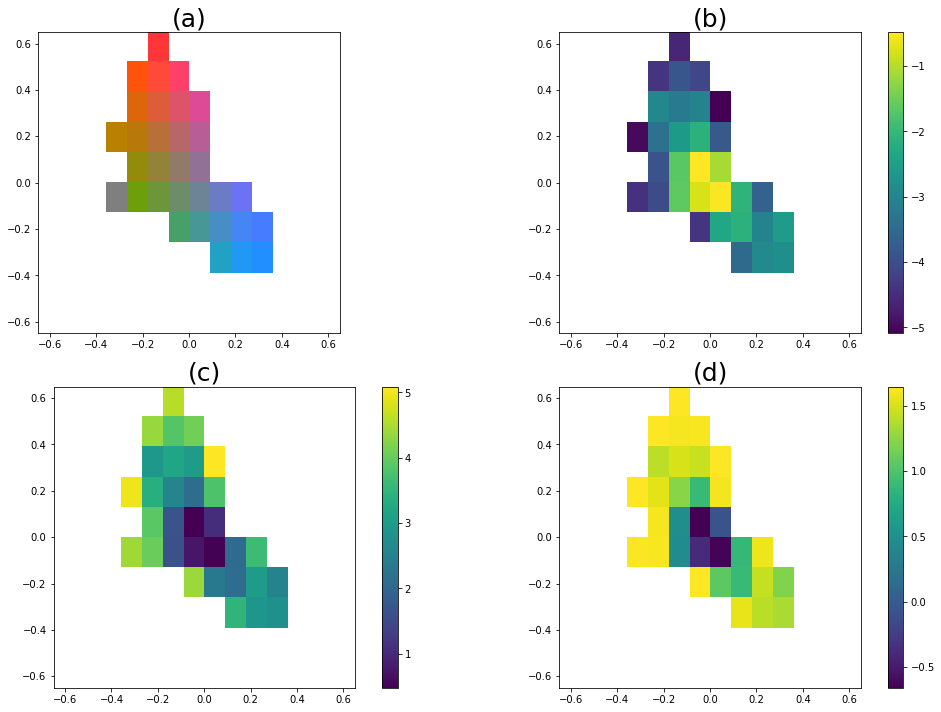
\includegraphics[width=200px]{cdexample.png}
\caption{(a) Color map, showing the mean color (\textit{chrominance}) of each of the selected bins (here, we set a threshold of 32 bins to select). (b) Frequency map (log-scale), shows the empirical frequency of the colors within each bin, computed over a dataset beforehand. (c) Inverse-frequency map (log-scale), \ie the inverse of (b). (d) Weight map (log-scale), shows the weights assigned to each bin after rebalancing. Interestingly, we notice that the amplitude in weights is much smaller than the amplitude in frequency (2 orders of magnitude against 4), which means that we partially make up for the underrepresentation bias and therefore encourage the prediction of rare colors.}
\label{cdex}
\end{center}
\end{figure}

Figure \ref{cdex} shows our discretized colorspace, as well as what the weights of the bins look like after rebalancing.

Our end model is a U-Net that has 3 downsampling groups of convolutional layers and 2 connections between hidden layers of the same size (we set aside the last and first layers of the downsampling process). 

Figure \ref{structure} summarizes the structure of the final network, that we refer as \textit{ColorUNet}. 

To find this final model, we have tried several architectures. We have begun by trying a simple "flat" convolutional network with 3 layers. However, this model gave very poor performance. Intuitively, what happens is that the spatial receptive field was not large enough to capture meaningful general shapes. 

Starting from this idea, we then implemented a second model, that is deeper, with 6 groups of convolutional layers. The structure is a \textit{bottleneck}, where 3 groups of layers downsample the image using a max pooling, and 3 groups of layers upsample the image. Using groups of 3x3 convolutional layers rather than bigger filters allows to have a large receptive field with fewer parameters. 

This network gave interesting results, but it was very unstable and slow to train, since it is quite deep. Furthemore, the quality of the output we get was not satisfying, even for a reduced task, because of this underfitting. Furthermore, the upsamopling process needs more filters in the hidden layers, as we need to encode more information to correctly upsample the image. 

Those observations led us to design our final \textit{ColorUNet}, that still has a bottleneck structure but uses connections between layers to improve the gradient flow, help the upsampling. We also added additional batch normalization layers to improve training stability. 

\begin{figure}
\begin{center}
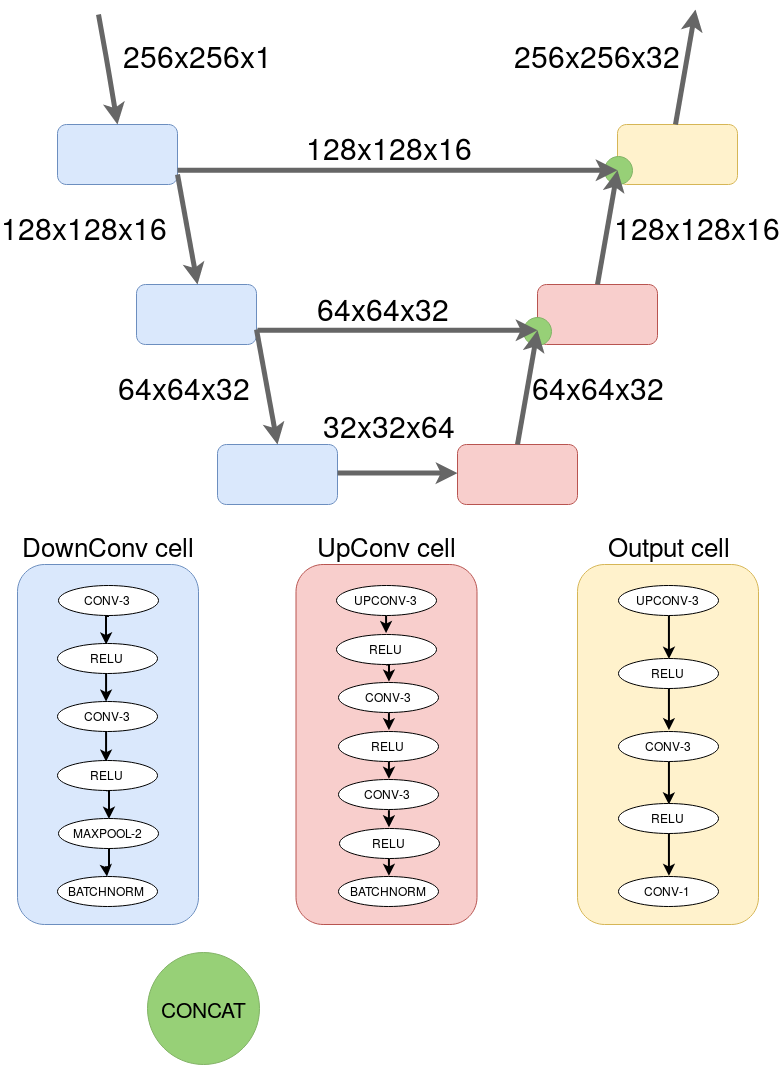
\includegraphics[width=200px]{diagram}
\caption{Structure of the \textit{ColorUNet}. We use 3 types of cells: DownConv Cells that use 2 stacked convolutional layers to have a large perceptive field and a maxpooling to downsample the image, UpConv cells that use 1 ConvTranspose Layer to upsample the image and then 2 convolutional layers, and an Output cell that is a simplified version of the UpConv cell}
\label{structure}
\end{center}
\end{figure}

\section{Dataset and Features}

\subsection{Datasets}
To train our model, we used subsets of the SUN \cite{xiao2010sun} and ImageNet \cite{russakovsky2015imagenet} datasets. We selected 8 categories from ImageNet and 14 categories from SUN, that correspond mainly to nature landscapes. Our final training set is composed of 13,469 images -- as a reference for comparison, \cite{zhang2016colorful} train their model on 1.5M+ images. Our validation set is made up of 2,889 images. A sample of the training data is shown in Figure \ref{sampletrain}.
We also tried training the model on the full SUN dataset (for only one epoch), to compare performance and gain insight on the importance for the model to go over the same examples several times to learn well.

\begin{figure}
\begin{center}
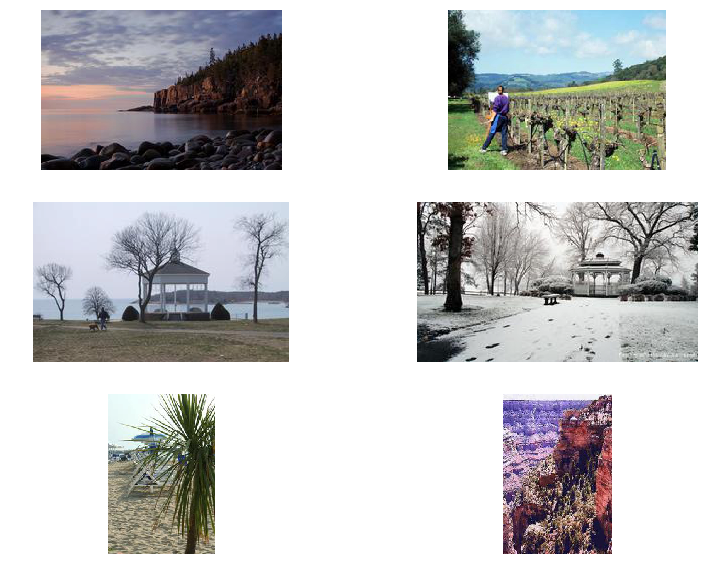
\includegraphics[width=200px]{sampletrain.png}
\caption{TODO}
\label{sampletrain}
\end{center}
\end{figure}

To keep a reasonable size for our tensors and have uniformity in our dataset, the images have all been downsampled to fit in a 256x256px frame (if downsampling was necessary). The downsampling has been performed using Lanczos method (with a $\text{sinc}$ kernel), and we used a mask for non-square images to make sure the loss is relevant. 

\subsection{Data Augmentation}

To improve the robustness of the model we train, we have implemented data augmentation. For each original image of the training set, we generate several training images by 
\begin{itemize}
\item Flipping the image along the horizontal axis
\item Adding noise to the image (with different intensities)
\item Selecting random crops of the image
\end{itemize}

We noticed an improvement of training stability and of the quality of our predictions when including the data augmentation in the pipeline, compared to when simply using more images for training (so the actual size of the training set is the same). In the case described above, the size of our training set is dilated sevenfold.

\section{Results and discussion}
\section{Conclusion and perspectives}
\section*{Contributions and acknowledgements}


{\small
\bibliographystyle{ieee}
\bibliography{references}
}

\end{document}
